\documentclass[a4paper,12pt]{article}
\usepackage[spanish]{babel}
\usepackage{listings,lstautogobble}
\usepackage{graphicx} 
\author{Leandro Nehemias Camperoz}
\title{MiniTP Shell, procesos e hilos}

\begin{document}
\maketitle
\newpage
\begin{enumerate}
\item \textbf{Shell y terminal.}\newline

  Si bien era posible escribir un script con menos lineas de codigo, decidi usar una sintaxis un poco mas entendible. Usando variables mas descriptivas sobre los archivos y comandos con los que se esta trabajando.\newline
  
  \begin{lstlisting}[language=Bash,autogobble=true,basicstyle=\fontsize{9}{12}\ttfamily]
    #!/bin/bash

    USUARIO=$(whoami)
    NOMBRE_DIRECTORIO=$1
    HOME_USUARIO=/home/$USUARIO/

    if [ $NOMBRE_DIRECTORIO ];then
        # Las siguientes lineas se ejecutan si se paso un parametro
        # NOMBRE_DIRECTORIO != ""
        NUEVO_DIRECTORIO=$HOME_USUARIO/$NOMBRE_DIRECTORIO
        NUEVO_ARCHIVO=$NUEVO_DIRECTORIO/contenido_home.txt
    
        mkdir $NUEVO_DIRECTORIO && touch $NUEVO_ARCHIVO
        # Volcamos la salida del comando ls en contenido_home.txt
        # [-l muestra permisos, tamano, usuario, fecha y hora de creacion] 
        # [-a no ignora archivos ocultos] [-v ordena por version ]
        # [--group-directories-first directorios primero]
        ls -lav --group-directories-first $HOME_USUARIO >\
        $NUEVO_ARCHIVO
    else
        echo "Error:Debe ejecutar con un parametro por lo menos."
        exit 1
    fi

    cat $NUEVO_ARCHIVO
    # Comando read
    # Solicitamos al usuario que presione una teclas o ingrese algun parametro
    # [-s no muestra caracteres ingresados ] [ -p muestra en pantalla mensaje ]
    # [-r barra invertida no escapa caracteres ]
    # Al leer la barra invertida como parte de lo que ingresa el usuario
    # solo termina de leer por teclado cuando presionamos [Enter].
    read -rsp $"Presione Enter para salir... \n" 
    exit 0
  \end{lstlisting}
  \newpage
\item \textbf{Estados de un proceso.}\newline
  
  Despues de varios intentos logre capturar el cambio de estado del proceso. El el codigo fuente del programa usado esta en proceso.c incluido en el archivo zip enviado.\newline
  
  Programa esperando input del usuario.\newline
  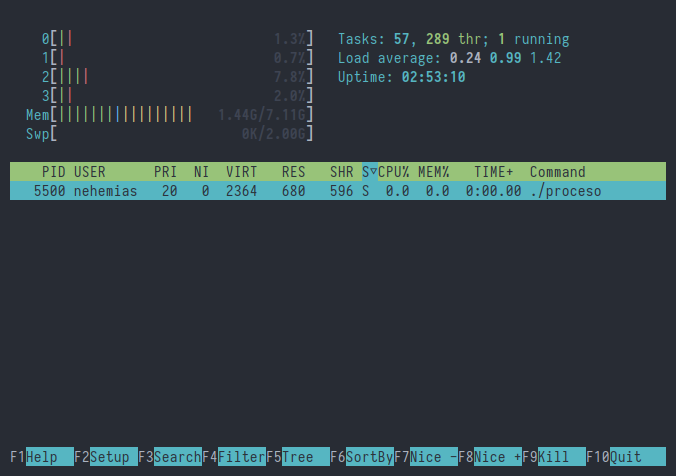
\includegraphics[width=10cm, height=7cm]{proceso1.png}

  \vspace{1.3cm}
  Programa realizando operaciones aritmeticas y mostrando por pantalla el resulatdo cada 1 microsegundo.\newline
  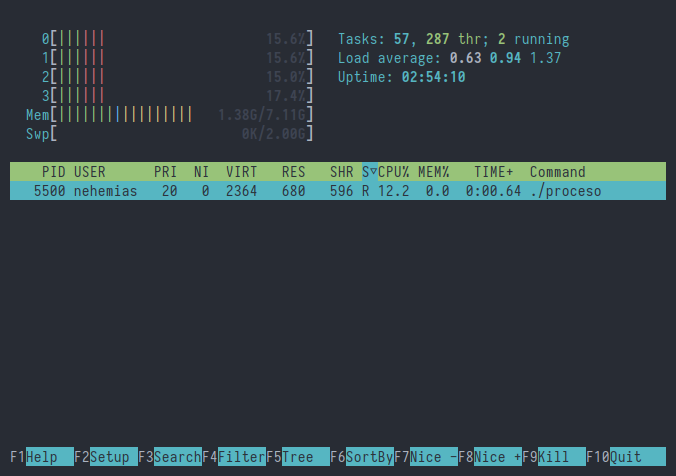
\includegraphics[width=10cm, height=7cm]{proceso2.png}
  \newpage
\item \textbf{Threads.}\newline

  Luego de modificar el codigo suministrado en el enunciodo del trabajo practico y ejecutar el programa. Obtuve como resultado una diferencia considerable en el tiempo de ejecucion. El codigo del programa utilizado esta en el archivo hilos.c.\newline

  Prueba realizada en un procesador intel i3 dual-core, con 2 LCPU por core, 2.3Ghz de frecuencia maxima.\newline
  
  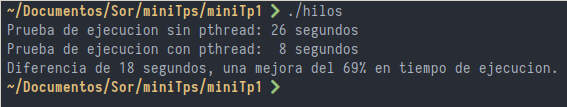
\includegraphics[width=9cm]{output_hilos.png}

  Captura htop, ejecucion del programa sin pthread.\newline
  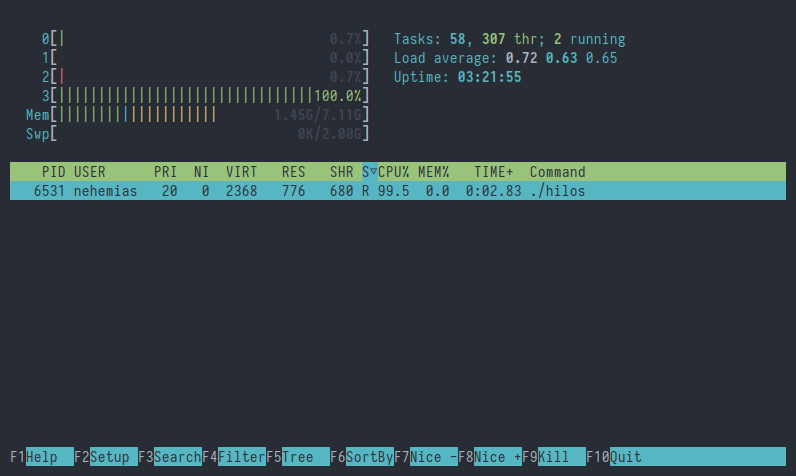
\includegraphics[width=9cm]{sin_pthread.png}

  Captura htop, ejecucion del programa con pthread.\newline
  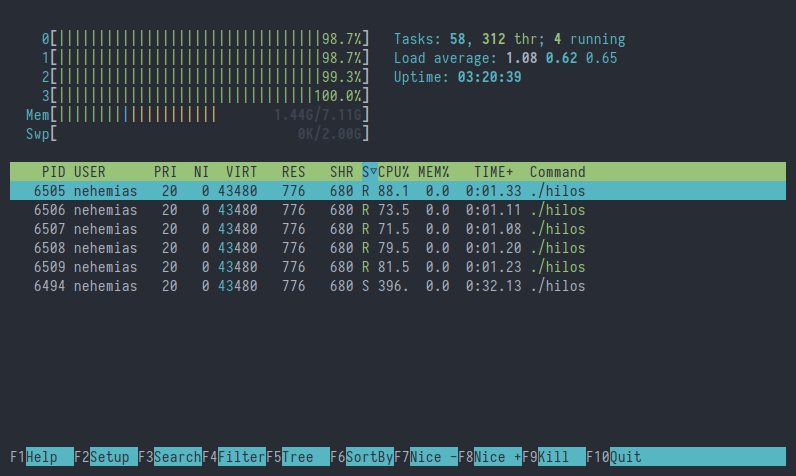
\includegraphics[width=9cm]{con_pthread.png}
\end{enumerate}
\end{document}

